%!TEX root = paper.tex
%%%%%%%%%%%%%%%%%%%%%%%%%%%%%%%%%%%%%%%%%%%%%%%%%%%%%%%%%%%%%%%%%%%%%%%%%%%%%%%%
\section{An End-to-End Lag Model}
\label{sec:model}

The proposed abstract lag model can be adapted to any gaming use case, be it either local, networked, or cloud games. Depending on the specific scenario, more or less components have to be factored in (e.g., the network path and game server with its discrete game ticks for an online game, or the video encoding and decoding elements in cloud gaming). Generally, it derives the \gls{E2E} lag from those factors, specifically including the framerate, tickrate, network \gls{QoS}, client/server messaging rates, and I/O characteristics. The \gls{E2E} lag is here defined to be the time elapsed between the player supplying commands to the input devices and the corresponding audio/video output. Figure~\ref{fig:queuing-model} depicts the overall queuing model.

\begin{figure*}[!t]
	\centering
	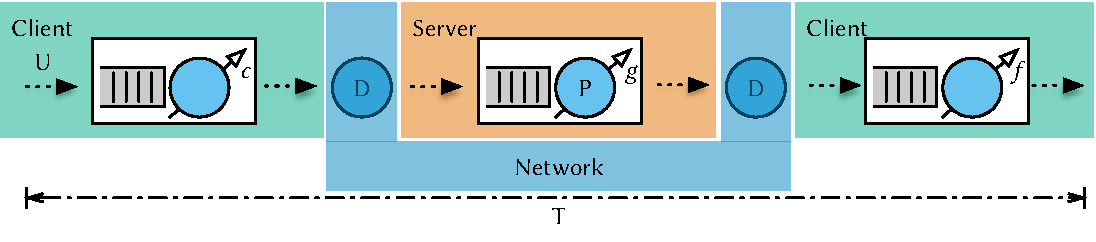
\includegraphics[width=1.0\textwidth]{../../../models/e2e-lag-model.pdf}
	\caption{Queuing lag model in an online video game case.}
\label{fig:queuing-model}
\end{figure*}




\begin{table}[!t]
\caption{Notation used in the model. Random variables are denoted by capital letters $X$, and constants by small letters $x$.}
\label{tab:notation}
	\centering
	\begin{tabu}{lX[1,l]X[1,l]}
	\toprule
	\textbf{Symbol} & \textbf{Description} & \textbf{Simulation} \\
	\midrule
	$D$ & network delay between game client and server & $D \sim TNorm(\mu_D;\sigma_D)$, $\mu_D = \SI{20}{\milli\second}$; $\sigma_D = \SI{5}{\milli\second}$\\
	$P$ & game server processing time & $P \sim TNorm(\mu_P;\sigma_P)$, $ \mu_P = \SI{3}{\milli\second}; \sigma_P = \SI{0.1}{\milli\second}$\\
	$T$ & end-to-end lag & key performance measure \\
	$U$ & (inter arrival) time between user inputs & $U \sim Exp(\lambda)$; $\lambda = \SI{50}{\milli\second}$\\
	\midrule
	$c$ & command rate & $c=g$ \\
	$c^{-1}$ & interval to gather input events before sending & \\
	$d$ & decode delay & \SI{5}{\milli\second} \\
	$e$ & encode delay & \SI{15}{\milli\second} \\
	$f$ & framerate & $f \in \SIrange{10}{200}{\hertz}$ \\
	$f^{-1}$ & frame duration & $f^{-1} \in \SIrange{5}{100}{\milli\second}$ \\
	$g$ & game tickrate & $g \in \SIrange{10}{200}{\hertz}$ \\
	$g^{-1}$ & game tick duration & $g^{-1} \in \SIrange{5}{100}{\milli\second}$ \\
	\bottomrule
	\end{tabu}
\end{table}



\begin{figure}[!t]
	\centering
	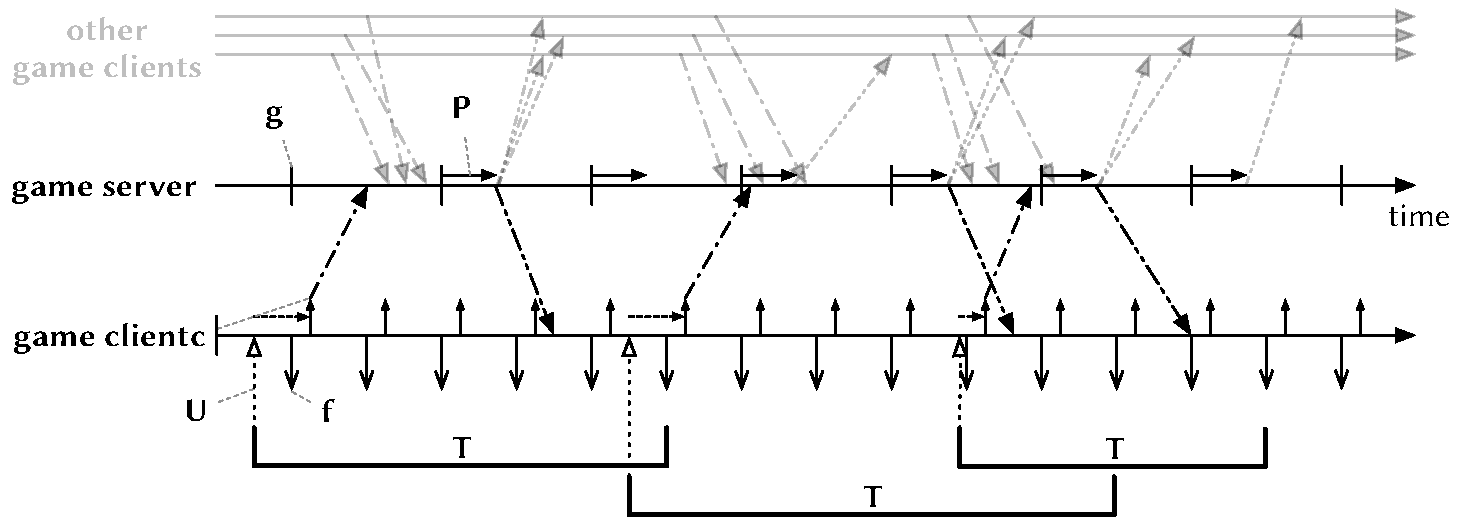
\includegraphics[width=1.0\columnwidth]{../../../models/tickrate-timeseries-notation.pdf}
	\caption{Exemplary flow of events in an online client-server game, and resulting end-to-end lag with the notation of Tab.~\ref{tab:notation}.
	% \hoss{Notation aus Tabelle ~\ref{tab:notation} waere gut im Bild. }
	} %Delay values are given for a framerate of \SI{60}{\hertz} and a server tickrate of \SI{30}{\hertz}, the network latency will only show minor variations.}
\label{fig:tickrate-timeseries}
\end{figure}
